\begin{figure}
    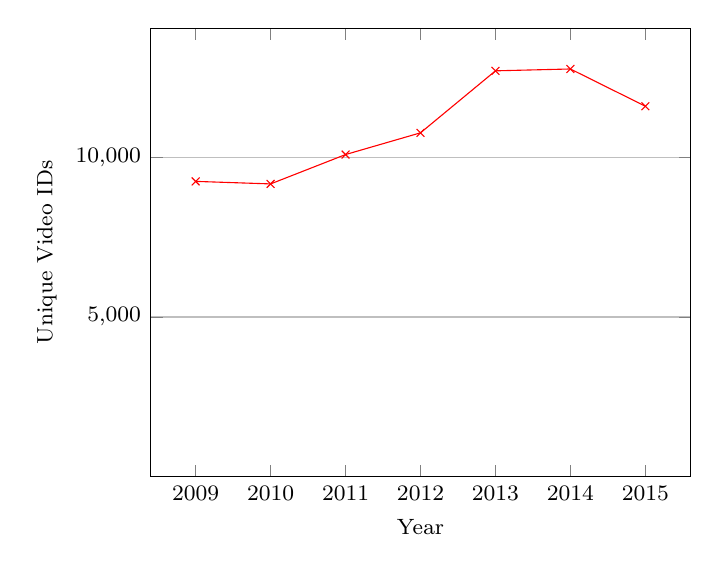
\begin{tikzpicture}
        \begin{axis}[
            ymin = 0,
            xlabel = Year,
            ylabel = Unique Video IDs,
            font = \footnotesize,
            xtick = {1, ..., 7},
            xticklabels = {2009, 2010, 2011, 2012, 2013, 2014, 2015},
            ytick = {5000, 10000},
            scaled y ticks = false,
            ymajorgrids = true
            ]
            \addplot[color=red, mark=x] coordinates {
                (1, 9248)
                (2, 9169)
                (3, 10089)
                (4, 10770)
                (5, 12712)
                (6, 12770)
                (7, 11603)
            };
       %     \addplot[color=blue, mark=*] coordinates {
       %         (1, 8793)
       %         (2, 9180)
       %         (3, 10038)
       %         (4, 8218)
       %         (5, 10205)
       %         (6, 11933)
       %         (7, 11603)
       %     };
        \end{axis}
    \end{tikzpicture}
    \captionof{figure}{Unique video IDs for January, by year}
    \label{jan-ids-year}
\end{figure}

